\documentclass[12pt,letterpaper]{article}
\usepackage{fullpage}
\usepackage[top=2cm, bottom=4.5cm, left=2.5cm, right=2.5cm]{geometry}
\usepackage{amsmath,amsthm,amsfonts,amssymb,amscd}
\usepackage{lastpage}
\usepackage{enumerate}
\usepackage{fancyhdr}
\usepackage{mathrsfs}
\usepackage{xcolor}
\usepackage{graphicx}
\usepackage{listings}
\usepackage{hyperref}
\usepackage{float}

\hypersetup{%
  colorlinks=true,
  linkcolor=blue,
  linkbordercolor={0 0 1}
}
 
\renewcommand\lstlistingname{Algorithm}
\renewcommand\lstlistlistingname{Algorithms}
\def\lstlistingautorefname{Alg.}

\lstdefinestyle{Python}{
    language        = Python,
    frame           = lines, 
    basicstyle      = \footnotesize,
    keywordstyle    = \color{blue},
    stringstyle     = \color{green},
    commentstyle    = \color{red}\ttfamily
}

\setlength{\parindent}{0.0in}
\setlength{\parskip}{0.05in}

% Edit these as appropriate
\newcommand\course{CS 470}
\newcommand\hwnumber{1}                  % <-- homework number
\newcommand\NetIDa{NetID: smarty}           % <-- NetID of person #1
\newcommand\NetIDb{STUID: 2283420}           % <-- NetID of person #2 (Comment this line out for problem sets)

\pagestyle{fancyplain}
\headheight 35pt
\lhead{\NetIDa}
\lhead{\NetIDa\\\NetIDb}                 % <-- Comment this line out for problem sets (make sure you are person #1)
\chead{\textbf{\Large Homework \hwnumber}}
\rhead{\course \\ \today}
\lfoot{}
\cfoot{}
\rfoot{\small\thepage}
\headsep 1.5em
% START
\begin{document}
\section*{Collaboration Statement}

The \LaTeX template I am using can be found on \textit{overleaf.com}.

I also used the \LaTeX   introduction website and  chatted with Katherine Walton, Luis Gomez Flores and Jack Frumkes about the assignment.

I made extensive use of the Python and Pandas documentation while completing this assigment. Stack Overflow was also very helpful.

I've included a Jupyter notebook with my solution. You're welcome to run it in the same folder as \textit{grades.csv}. It loads the file in a Pandas DataFrame and performs all the data manipulations for this assignment.

\section*{Task 1: Attribute Description}

\begin{itemize}
    \item 
    Semester: currently \textit{categorical}, represents the semester during which the student took this course. This probably should be \textit{ordinal}, as there is a clear chronological order between semesters
    \item
    Student ID: \textit{categorical}, identifies a student in the Emory system. 
    \item
    Name: \textit{categorical}, the first name of the student
    \item
    Section: \textit{categorical}, the section of CS170 the student is in.
    \item
    Homework 1-5: \textit{numerical ratio}, the grade for a given student for each homework. The maximum grade is 42 for each homework (40 + 2 bonus points for submitting early).
    \item
    Peer Evaluation: \textit{numerical ratio}, the sum of the peer evaluation points earned by a student. The maximum score is 150
    \item
    Bonus: \textit{numerical ratio}, most students do not have a value for this attribute. This represents the number of Bonus points a student earned.
    \item
    Quiz 1-12: \textit{numerical ratio}, the grade for a given student for each quiz. The maximum grade for one quiz is 50.
    \item
    Quiz Adjustment: \textit{numerical ratio}. This represents an adjustment to the quiz grade for exceptional purposes (I'm guessing a makeup or regrade) 
    \item
    Drop Lowest Quiz 1-2: \textit{numerical ratio}, opposites of the two lowest scores of the student, so that they cancel out those scores when added up.
    \item
    Final Exam: \textit{numerical ratio}, final exam score, out of 150.
    \item
    Total Score: \textit{numerical ratio}: sum of all previous numerical columns, represents the final score of a student out of 1000.
    \item
    Letter Grade: \textit{ordinal}, equivalent letter grade according to the table in the syllabus.
\end{itemize}

\section*{Task 2: Missing Values}

\begin{itemize}
    \item 
    \textbf{Homework 1-5}: It seems some people forgot to submit their homework... In most classes, the student would probably end up getting a zero for the given assignment (we fill the null value with a zero). If there are extraneous circumstances (illness, etc.) or we are very lenient, I suppose we could replace the null value with the average of the other homework assignments for that student. This however assumes that the student would perform as well on that missing homework as on the others, which is often not the case as assignments can vary greatly in breadth and depth throughout the semester. I'm leaning more towards filling with zeroes.
    \item
    \textbf{Peer evaluations}: The missing entries here could either be due to a student not completing ONE peer evaluation, or not completing ANY peer evaluations throughout the semester. If it's the latter, we can simply zero-fill the null values for the same reasons as \textbf{Homework 1-5}. 
    
    After further looking at the data, it appears the vast majority of the people that had a null value in this field failed the course. Maybe these students withdrew from the course? In that case, it might be safer to delete their entries from the table, as these students are not representative of students that completed CS170. They should be analyzed separately (maybe this can allow us to discover some shortcomings in the course, or to find where students struggle the most).
    \item
    \textbf{Bonus}: 769 students do not have an entry for this field (this is much higher than for other attributes). This makes sense as the bonus is, by definition, optional. We can just fill null values with zeroes here. Other options do not really make sense.
    \item
    \textbf{Quiz 1-10}: The student most likely did not show to the quiz. We can fill this field with a zero. If the student made up the quiz, it will be reflected in the "Quiz Adjustment" Attribute.
    \item
    \textbf{Quiz Adjustment}: Most students don't need their quiz grade adjusted. The vast majority of students don't have an entry here. Filling in with zeroes makes most sense for this field.
    \item
    \textbf{Final Exam}: It appears some people did not take the final exam. It might be because they were taking the class pass-fail and could pass the class even if they got a zero on the final, or they dropped the course, or missed the exam. Filling in this field with zeroes makes most sense for the same reasons as explained previously.
\end{itemize}

\section*{Task 3: Re-encoding}

\begin{itemize}
    \item 
    \textbf{Semester} can be separated in two attributes: \textit{Year} and \textit{Semester}, where
    
\begin{center}
 \begin{tabular}{| c |} 
 \hline
 Semester \\ [0.5ex] 
 \hline\hline
  F18 \\
  \hline
 S18 \\
 \hline
 F17 \\
 \hline
 F16 \\
 \hline
\end{tabular}

becomes
\vspace{1ex}

 \begin{tabular}{| c c |} 
 \hline
 Year & Fall/Spring \\ [0.5ex] 
 \hline\hline
  18 & F \\
  \hline
 18 & S \\
 \hline
 17 & F \\
 \hline
 16 & F \\
 \hline
\end{tabular}

\end{center}

This way, we can easily compare all fall semesters against all spring semesters for CS170.

\item
\textbf{Section} is currently denoted by a number. Someone could assume that the section number is ordinal (1 is somehow ranked either higher or lower than 9. Furthermore, section 2 for the fall 2018 semester is not necessarily the same as section 2 for the spring 2016 semester. This can become important if we are trying to evaluate the performance of lab TAs for a semester. For this reason, I will concatenate the semester value with the section value

For example:

\begin{verbatim}
    5
\end{verbatim}

Becomes:

\begin{verbatim}
    2018F-section5
\end{verbatim}
\end{itemize}
\section*{Task 4: Scaling and z-scoring}

\begin{enumerate}
    \item Re-scaling is most appropriate to help readers of the data get an idea of what the grade represents. Most people are familiar with the 0-100 grading scale and can quickly estimate what letter grade a student got for an assignment.
    \item Z-scoring using the mean of all semesters is only appropriate to do if the score distribution for each semester is homogeneous: if professors started grading harder in 2017, for example, the mean grade for each assignment would be skewed left. This would affect the z-scores of students who took the class before the grading change, and make them appear as better than their classmates from 2017 onwards.
    \item This Z-Scoring method is most appropriate if there can be significant disparity in grading methods from one semester to the other. Overall, this should be the preferred method of calculating z-scores with this dataset.
\end{enumerate}{}

\section*{Task 5: Summary Statistics}

Summary statistics were computed for each attribute and included in \textit{summary\_statistics.csv}.
% Rest of the work..

\section*{Task 7: Tools and Languages}

Please find Task 6 at the bottom of the document.

\begin{itemize}
    \item Python: General purpose programming language. I used this because I am familiar with it. It's easy and fast to write in. This is one of the most commonly used programming languages in data science.
    \item Pandas: A data manipulation library for Python. Pretty high learning curve compared to regular Python, but very powerful.
    \item matplotlib: A graphing library for python. Definitely more difficult to use than Excel graphing tools, but provides more rigid formatting.
    \item \LaTeX: Typesetting language with which this document was made. High learning curve. Using a pre-made template made this tool easier to use.
\end{itemize}

Tools I considered using but did not use
\begin{itemize}
    \item SQL: I am rather familiar with it, but did not have the time to set up a database with rules 
    \item R: Similar to Python with pandas and other Data Science libraries. I'm more familiar with the Python syntax and did not have time to study up on R.
\end{itemize}

\section*{Part 8: LaTeX Document}

NB: The code for this assignment is included in a separate Jupyter notebook for readability's sake.

\section*{Task 6: Charts}

\begin{figure}[!htb]
  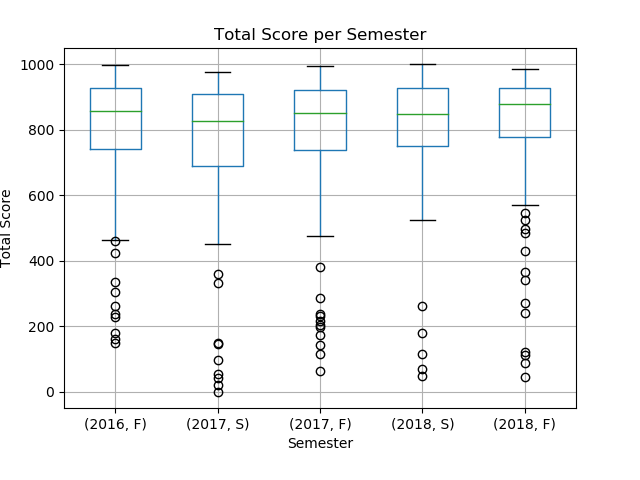
\includegraphics[width=\linewidth]{graph0.png}
  \caption{The Distribution of Total Scores for all sections for a given semester. Most semesters, the Total score distribution hovers around the low to mid 80s, which is expected from a college introduction course in computer science. The top 50\% of students appears to have a lesser range of scores than the bottom 50\%. Note the median total score appears to dip in the Spring of 2017, but then steadily seems to rise again. This could indicate some unforseen event that affected the students' ability to learn course material (Professor often missing that semester, Excessively difficult exams...) assuming student performance is relatively constant from one year to the next.}
\end{figure}

\begin{figure}[!htb]
  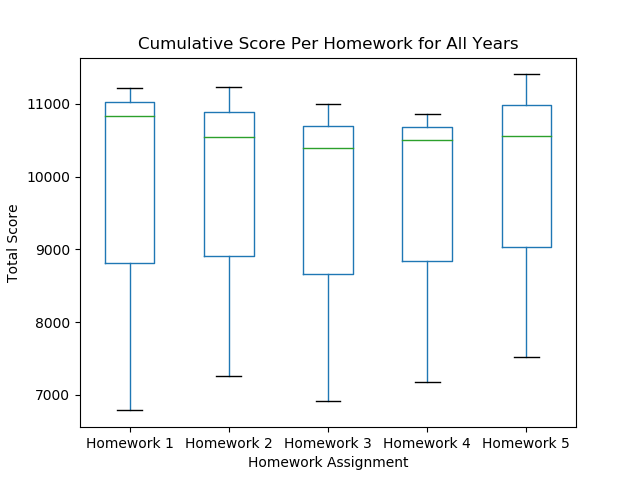
\includegraphics[width=\linewidth]{graph1.png}
  \caption{The sum of all student grades for a given homework assignment, per year. Note the grade range for the top 50\% of students is extremely small compared to the bottom 50\%. This suggests that there exists some significant disparity in student ability from year to year (This will be investigated further in another Figure). Median scores decrease until the middle of the semester (Homework 3), then increase again towards the end. This could suggest students are better assimilating the material as the class progresses. This could also indicate that students are unable to perform at their best during the middle of the semester. This would make sense considering this is when most students find themselves overwhelmed with the amount of homework assigned}
\end{figure}

\begin{figure}[!htb]
  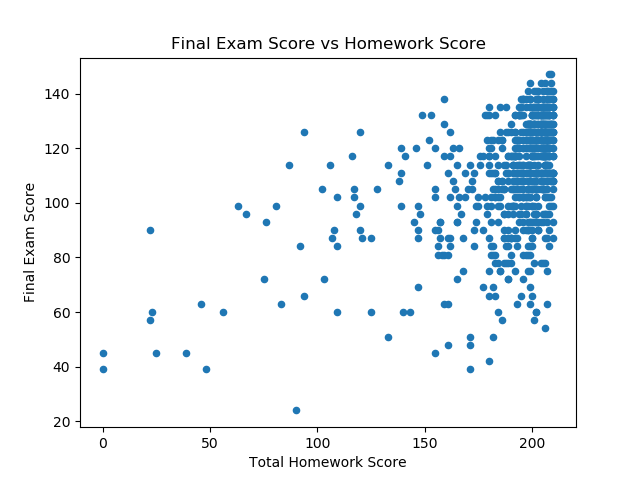
\includegraphics[width=\linewidth]{graph2.png}
  \caption{Final Exam Scores over Total Homework Scores per student that has taken CS170. The graph displays a moderately strong, positive correlation between Final Exam Score and Total Homework Score: Individuals that perform well on their homework assignments tend to do better on the Final Exam.
  }
\end{figure}

\begin{figure}[!htb]
  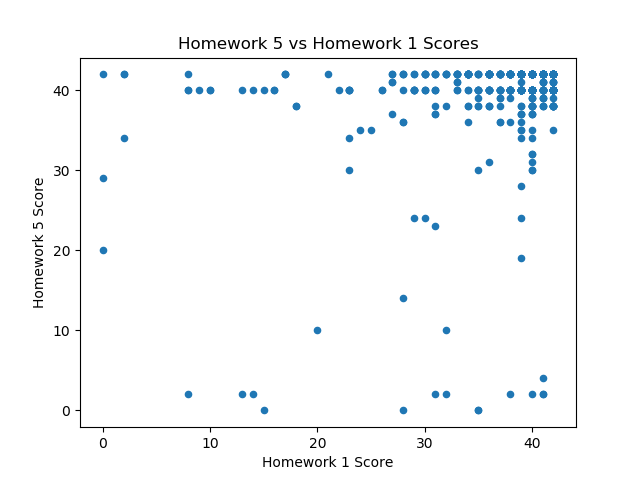
\includegraphics[width=\linewidth]{graph3.png}
  \caption{Comparison of Homework 1 and Homework 5 scores for every student. The objective of this graph is to observe any change in the performance of the student as the CS170 class progressed. It appears that students that performed well on the first Homework also performed well on the last Homework. A significant amount of students performed much better on their last homework than their first: this could be due to having better assimilated the class material after an entire semester.}
\end{figure}

\begin{figure}[!htb]
  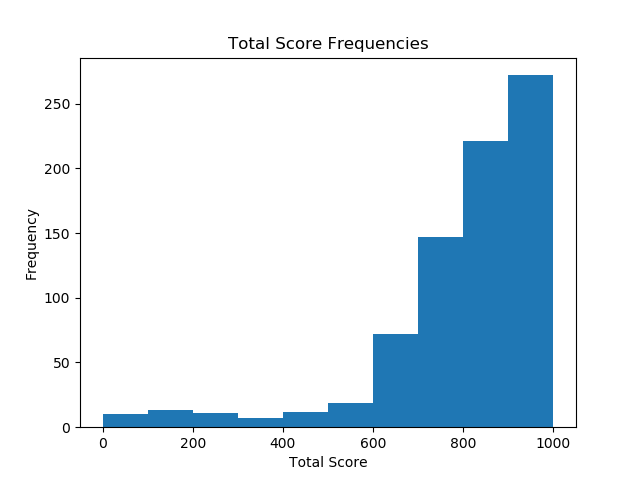
\includegraphics[width=\linewidth]{graph4.png}
  \caption{Frequencies of Total Scores for all years and sections. The distribution is highly skewed to the right, with most students scoring above 600 (passing the course). More students got A and A-s than any other letter grade in the course.}
\end{figure}

\begin{figure}[!htb]
  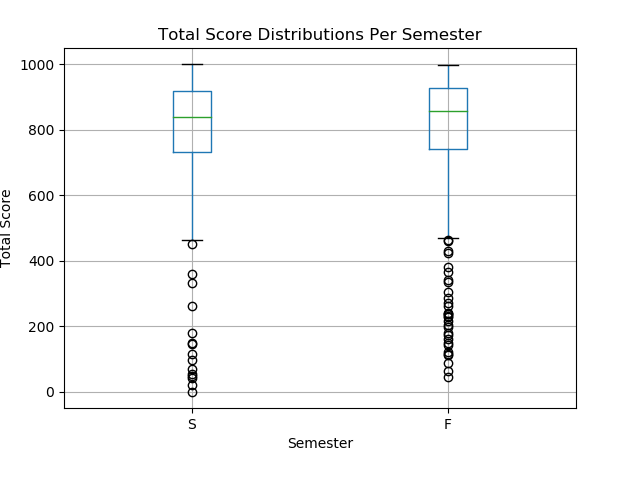
\includegraphics[width=\linewidth]{graph5.png}
  \caption{A comparison of Total Score Distribution for the Spring and the Fall Semesters. Both distributions display similarly shaped box plots. The median of the Spring distribution is slightly lower than that of the Fall distribution. This could be due to the fact that most Spring courses are somewhat faster paced than their Fall counterparts (professors dive faster into the material than in the Fall).}
\end{figure}

\begin{figure}[!htb]
  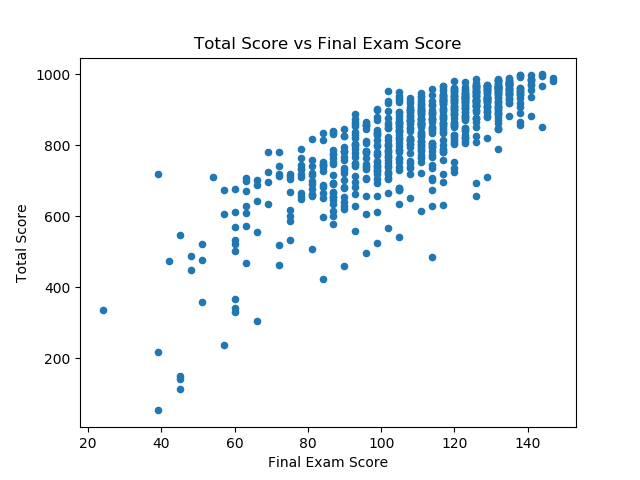
\includegraphics[width=\linewidth]{graph6.png}
  \caption{How Final Exam Score affect Total Score. Note that Final Exam Score only represents 15\% of a student's total score for CS170. However, the correlation coefficient between the two is surprisingly high regardless (0.88), which suggests that Final Exam Score is a good predictor of a student's total score in the class.}
\end{figure}

\begin{figure}[!htb]
  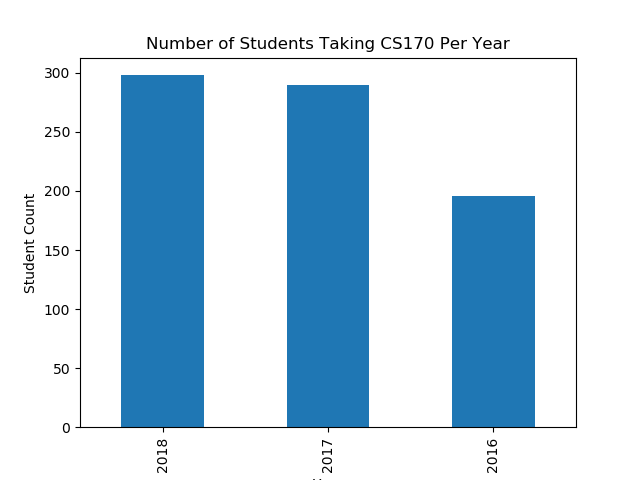
\includegraphics[width=\linewidth]{graph7.png}
  \caption{Student count per year for CS170. Note the number of students in CS170 has greatly increased over the years. This is most likely due to the increased popularity of Computer Science and its increased use in other fields (Mathematics, Physics, etc. but also Social Sciences). Around 300 people took CS170 in 2018.}
\end{figure}

\begin{figure}[!htb]
  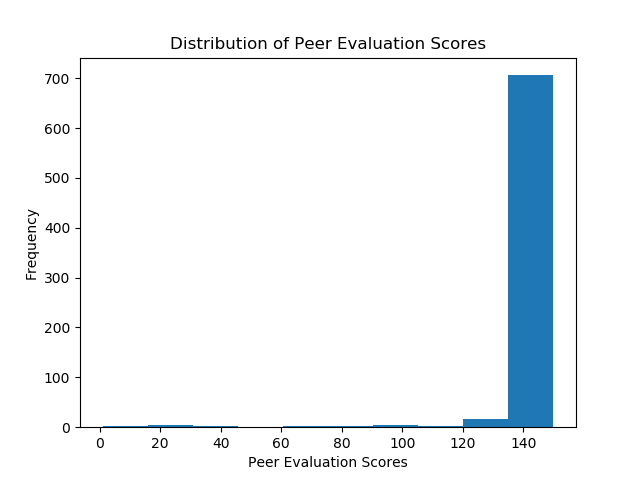
\includegraphics[width=\linewidth]{graph8.png}
  \caption{Peer Evaluation Scores for all years. The distribution is extremely skewed towards the right, suggesting the task is graded rather leniently}
\end{figure}

\begin{figure}[!htb]
  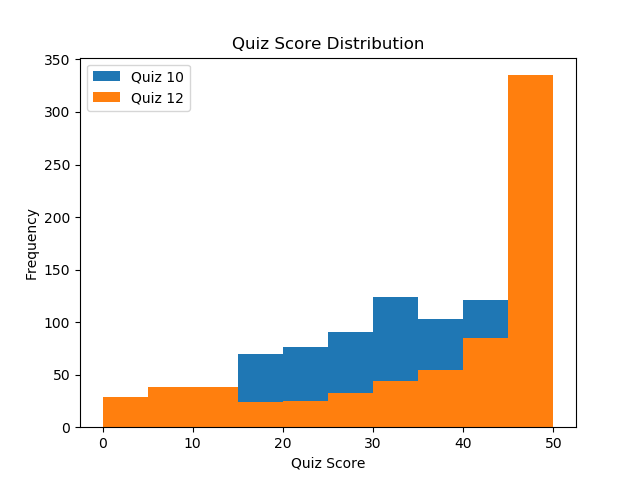
\includegraphics[width=\linewidth]{graph9.png}
  \caption{Comparison of Quiz 10 and Quiz 12 grades. Quiz 10, like many quiz distributions from the middle of the semester, has a very wide range of grades, with no grade being more common than another. Quiz 12, from the end of the semester, is extremely highly skewed towards the A range, which suggests this quiz was rather easy, maybe given as a grade booster to students before their final exam.}
\end{figure}
\end{document}
